\section{Object 6}
\markright{Object 6}

This object demonstrates the use of multiple feature types to build a complex part. The process began with creating and extruding the main base. Subsequently, a revolved feature was used to create circular geometry on two diagonal corners. To finalize the part, applied features were used: a Fillet was added to round a top edge, and a Chamfer was applied to create a beveled bottom edge, showcasing how different tools are combined in modeling.

\begin{figure}[H]
  \centering

  \begin{subfigure}[b]{0.49\textwidth}
    \centering
    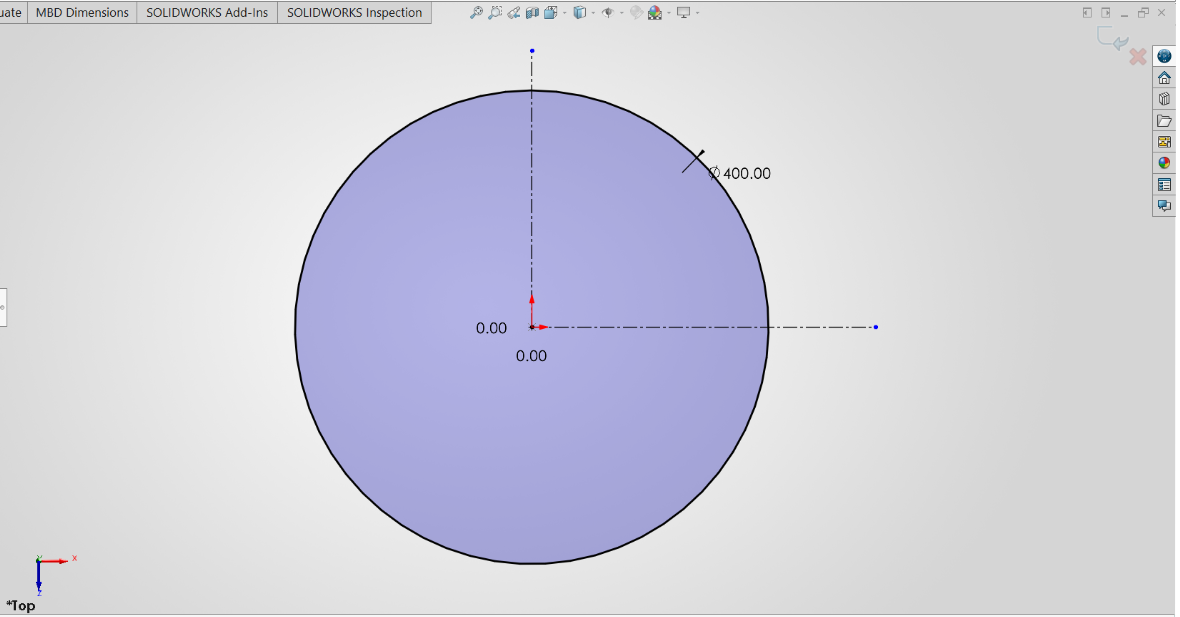
\includegraphics[width=\textwidth, keepaspectratio]{lab-01/assets/object-6/object-6-snap-1.png}
    \caption{2D sketch of the base with dimensions.}
  \end{subfigure}%
  \hfill
  \begin{subfigure}[b]{0.49\textwidth}
    \centering
    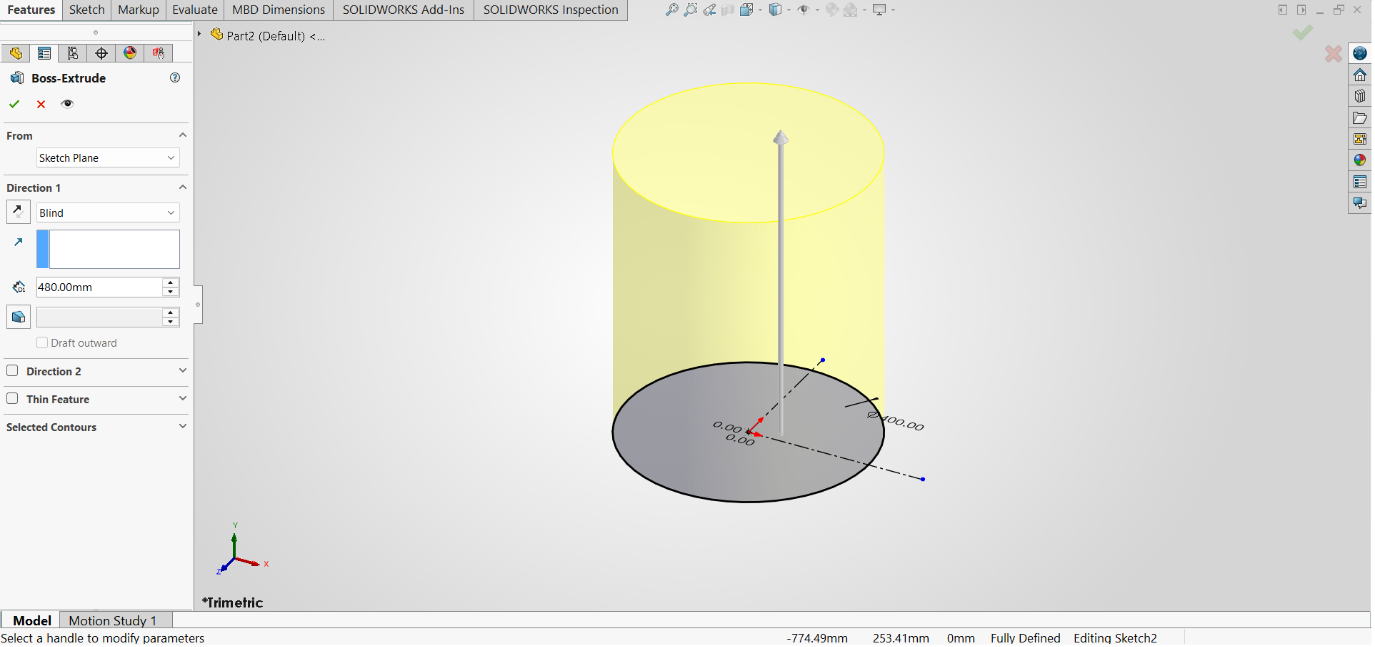
\includegraphics[width=\textwidth, keepaspectratio]{lab-01/assets/object-6/object-6-snap-2.png}
    \caption{Extruding the base sketch.}
  \end{subfigure}%
  \vspace{0.5em}
  \begin{subfigure}[b]{0.32\textwidth}
    \centering
    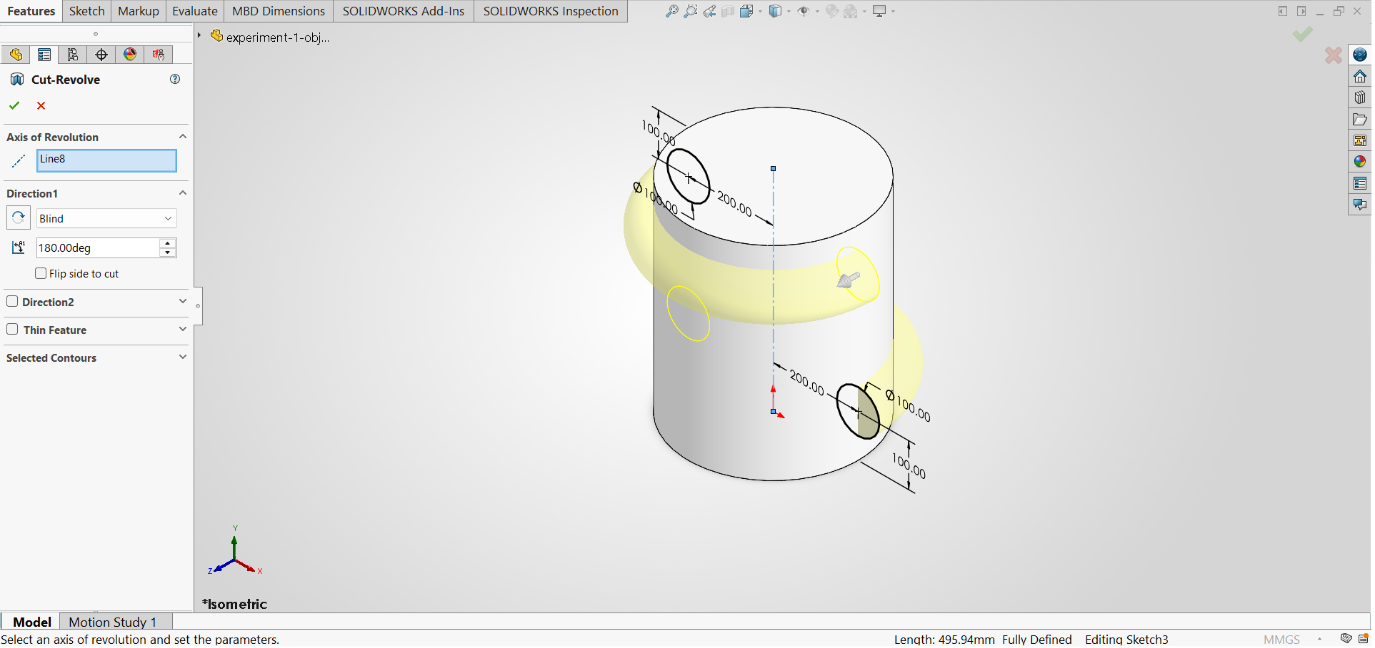
\includegraphics[width=\textwidth, keepaspectratio]{lab-01/assets/object-6/object-6-snap-5.png}
    \caption{Creating revolved features on diagonal corners.}
  \end{subfigure}%
  \hfill
  \begin{subfigure}[b]{0.32\textwidth}
    \centering
    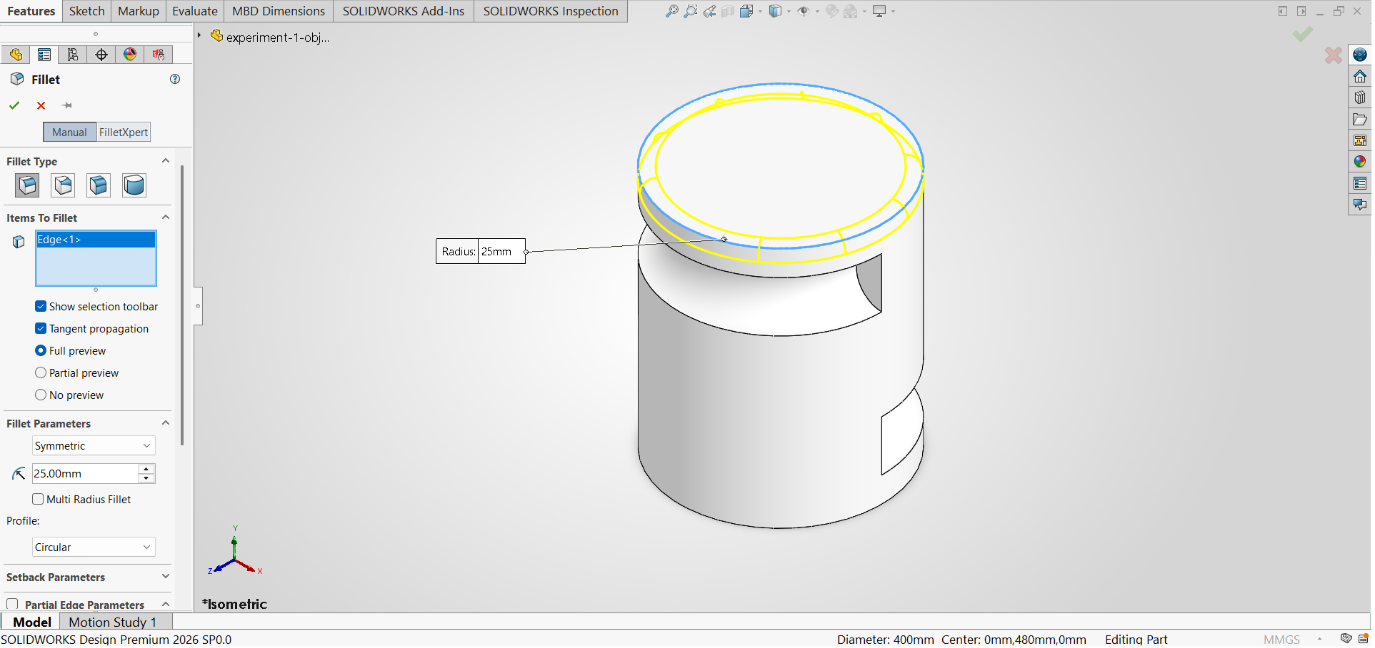
\includegraphics[width=\textwidth, keepaspectratio]{lab-01/assets/object-6/object-6-snap-7.png}
    \caption{Applying a Fillet feature to the top edge.}
  \end{subfigure}%
  \hfill
  \begin{subfigure}[b]{0.32\textwidth}
    \centering
    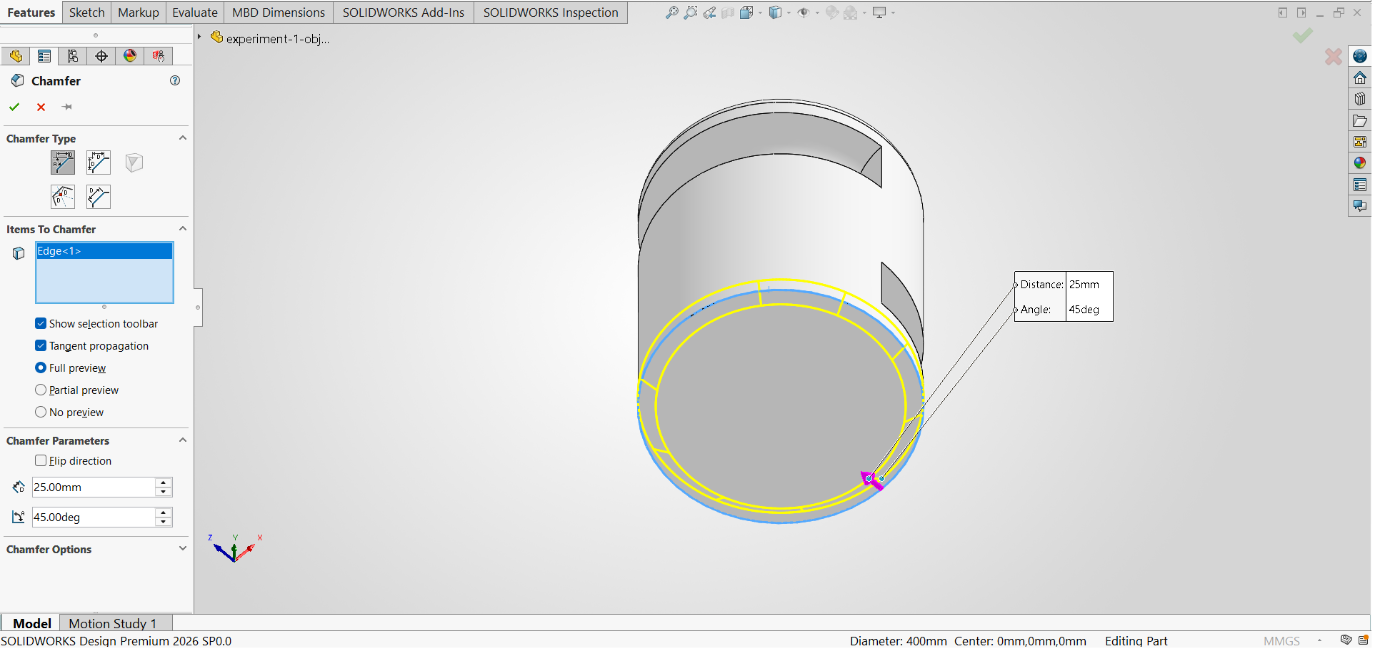
\includegraphics[width=\textwidth, keepaspectratio]{lab-01/assets/object-6/object-6-snap-9.png}
    \caption{Applying a Chamfer feature to the bottom edge.}
  \end{subfigure}%
  \vspace{0.5em}
  \begin{subfigure}[b]{\textwidth}
    \centering
    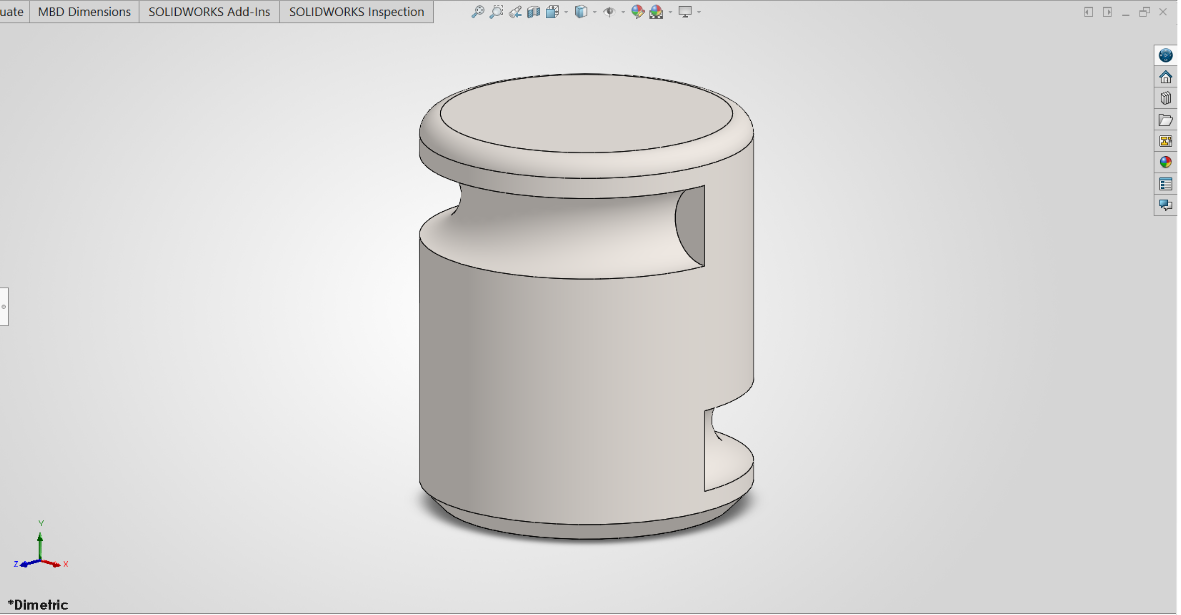
\includegraphics[width=\textwidth, keepaspectratio]{lab-01/assets/object-6/object-6-snap-10.png}
    \caption{Final Result.}
  \end{subfigure}

  \caption{Snapshots while Designing Object 6 in Solidworks}
  \label{lab01_object_6}
\end{figure}
